% Figure 5.4: DAPT Counter-Experiment
% PhoBERT Original vs PhoBERT + DAPT

\documentclass[border=5pt]{standalone}
\usepackage[utf8]{inputenc}
\usepackage{pgfplots}
\usepackage{helvet}
\usepackage[T1]{fontenc}

\pgfplotsset{
    width=13cm,
    height=7cm,
    compat=1.18,
}

\begin{document}
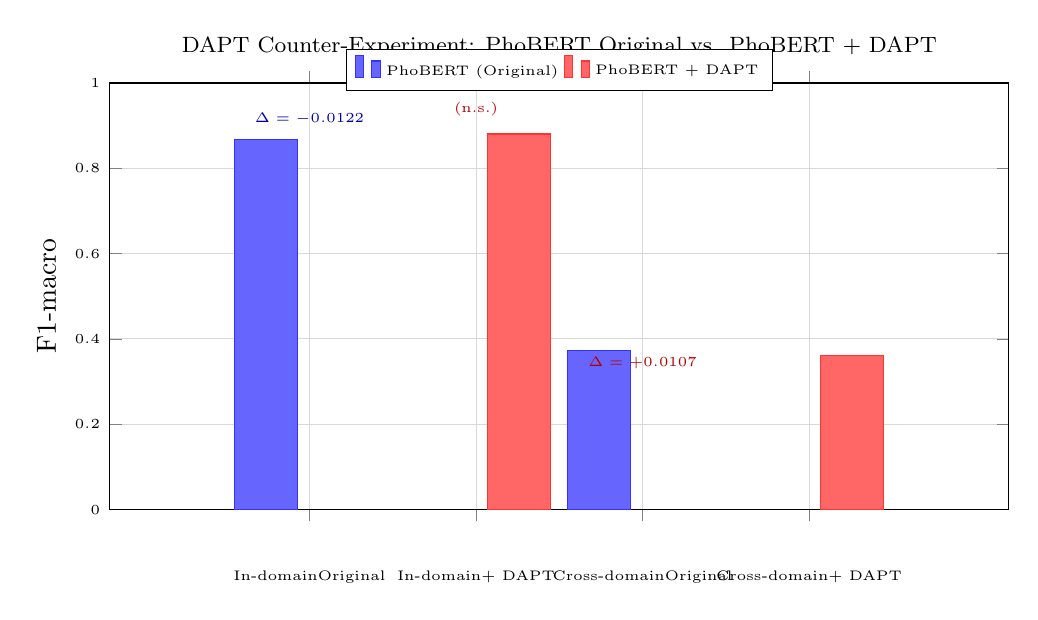
\begin{tikzpicture}
\begin{axis}[
    width=13cm,
    height=7cm,
    ybar=0.3cm,
    bar width=0.8cm,
    enlarge x limits=0.4,
    ymin=0, ymax=1,
    ylabel={F1-macro},
    title={DAPT Counter-Experiment: PhoBERT Original vs. PhoBERT + DAPT},
    title style={font=\footnotesize},
    tick label style={font=\tiny},
    grid=major,
    grid style={gray!30},
    ytick distance=0.2,
    xtick={1,2,3,4},
    xticklabels={
        {In-domain\\Original},
        {In-domain\\+ DAPT},
        {Cross-domain\\Original},
        {Cross-domain\\+ DAPT}
    },
    x tick label style={rotate=0, anchor=north, yshift=-0.5cm},
    cycle list={
        {fill=blue!60,draw=blue!80},
        {fill=red!60,draw=red!80},
    },
    legend style={
        at={(0.5,1.08)},
        anchor=north,
        legend columns=2,
        font=\tiny
    },
]

% Original models (blue)
\addplot coordinates {
    (1, 0.8681)
    (3, 0.3727)
};
\addlegendentry{PhoBERT (Original)}

% DAPT models (red)
\addplot coordinates {
    (2, 0.8803)
    (4, 0.3620)
};
\addlegendentry{PhoBERT + DAPT}

% Annotations
\node[anchor=south, font=\tiny, blue!70!black] at (axis cs:1,0.88) {$\Delta = -0.0122$};
\node[anchor=south, font=\tiny, red!70!black] at (axis cs:2,0.90) {(n.s.)};
\node[anchor=north, font=\tiny, red!70!black] at (axis cs:3,0.38) {$\Delta = +0.0107$};

\end{axis}
\end{tikzpicture}
\end{document}
